\documentclass[12pt]{article}
\usepackage{amsmath}
\usepackage{amssymb}
\usepackage{enumitem}
\usepackage{graphicx}
\usepackage{hyperref}
\usepackage{tikz}

\title{CS461 Homework 3}
\author{Mannan Shukla}
\date{Due: Nov. 19, 11:59 PM}

\begin{document}

\maketitle

\section*{1. Decision Tree}
\section*{1.1 Information Gain and Root Node Selection}

The initial entropy of the $\text{Play}$ is: $H(Play) = 1.0000$

\begin{itemize}
    \item \textbf{Weather:} $IG(\text{Weather}) = 0.4000$
    \item \textbf{Temperature:} $IG(\text{Temperature}) = 0.1145$
    \item \textbf{Humidity:} $IG(\text{Humidity}) = 0.0349$
    \item \textbf{Wind:} $IG(\text{Wind}) = 0.1245$
\end{itemize}

\noindent Since \textbf{Weather} has the highest Information Gain $0.4000$, it is selected as the root node of the decision tree.

\begin{center}
    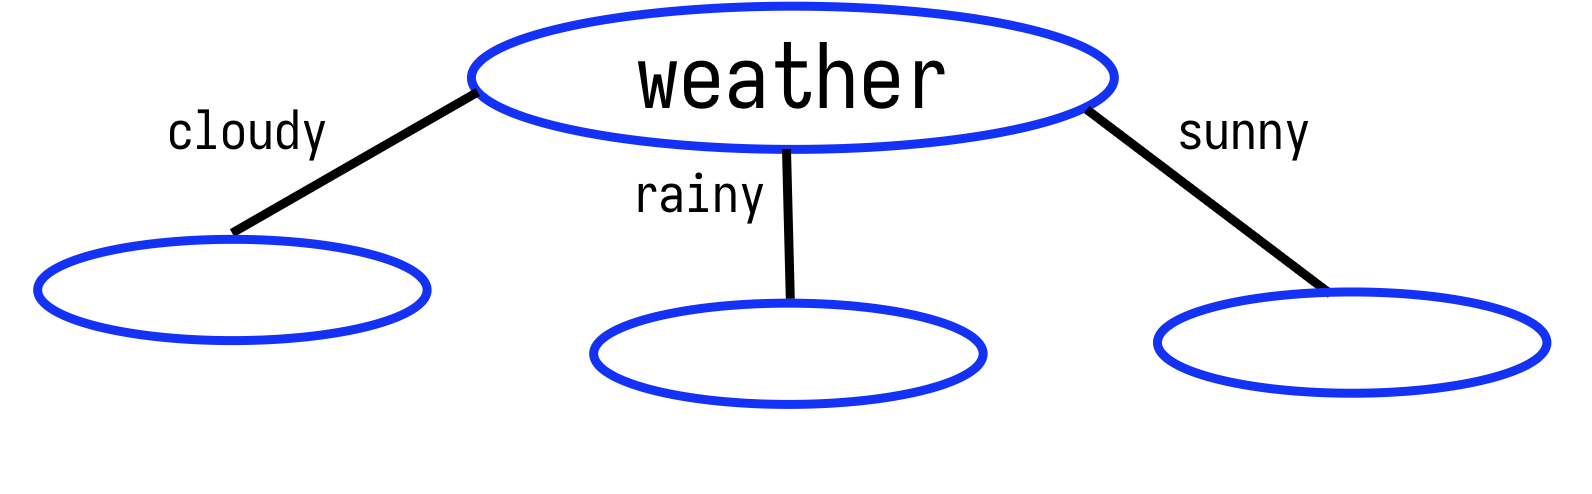
\includegraphics[width=0.8\textwidth]{1.png}
\end{center}

\section*{1.2 Constructing the Decision Tree}

The decision tree is shown below:

\begin{center}
    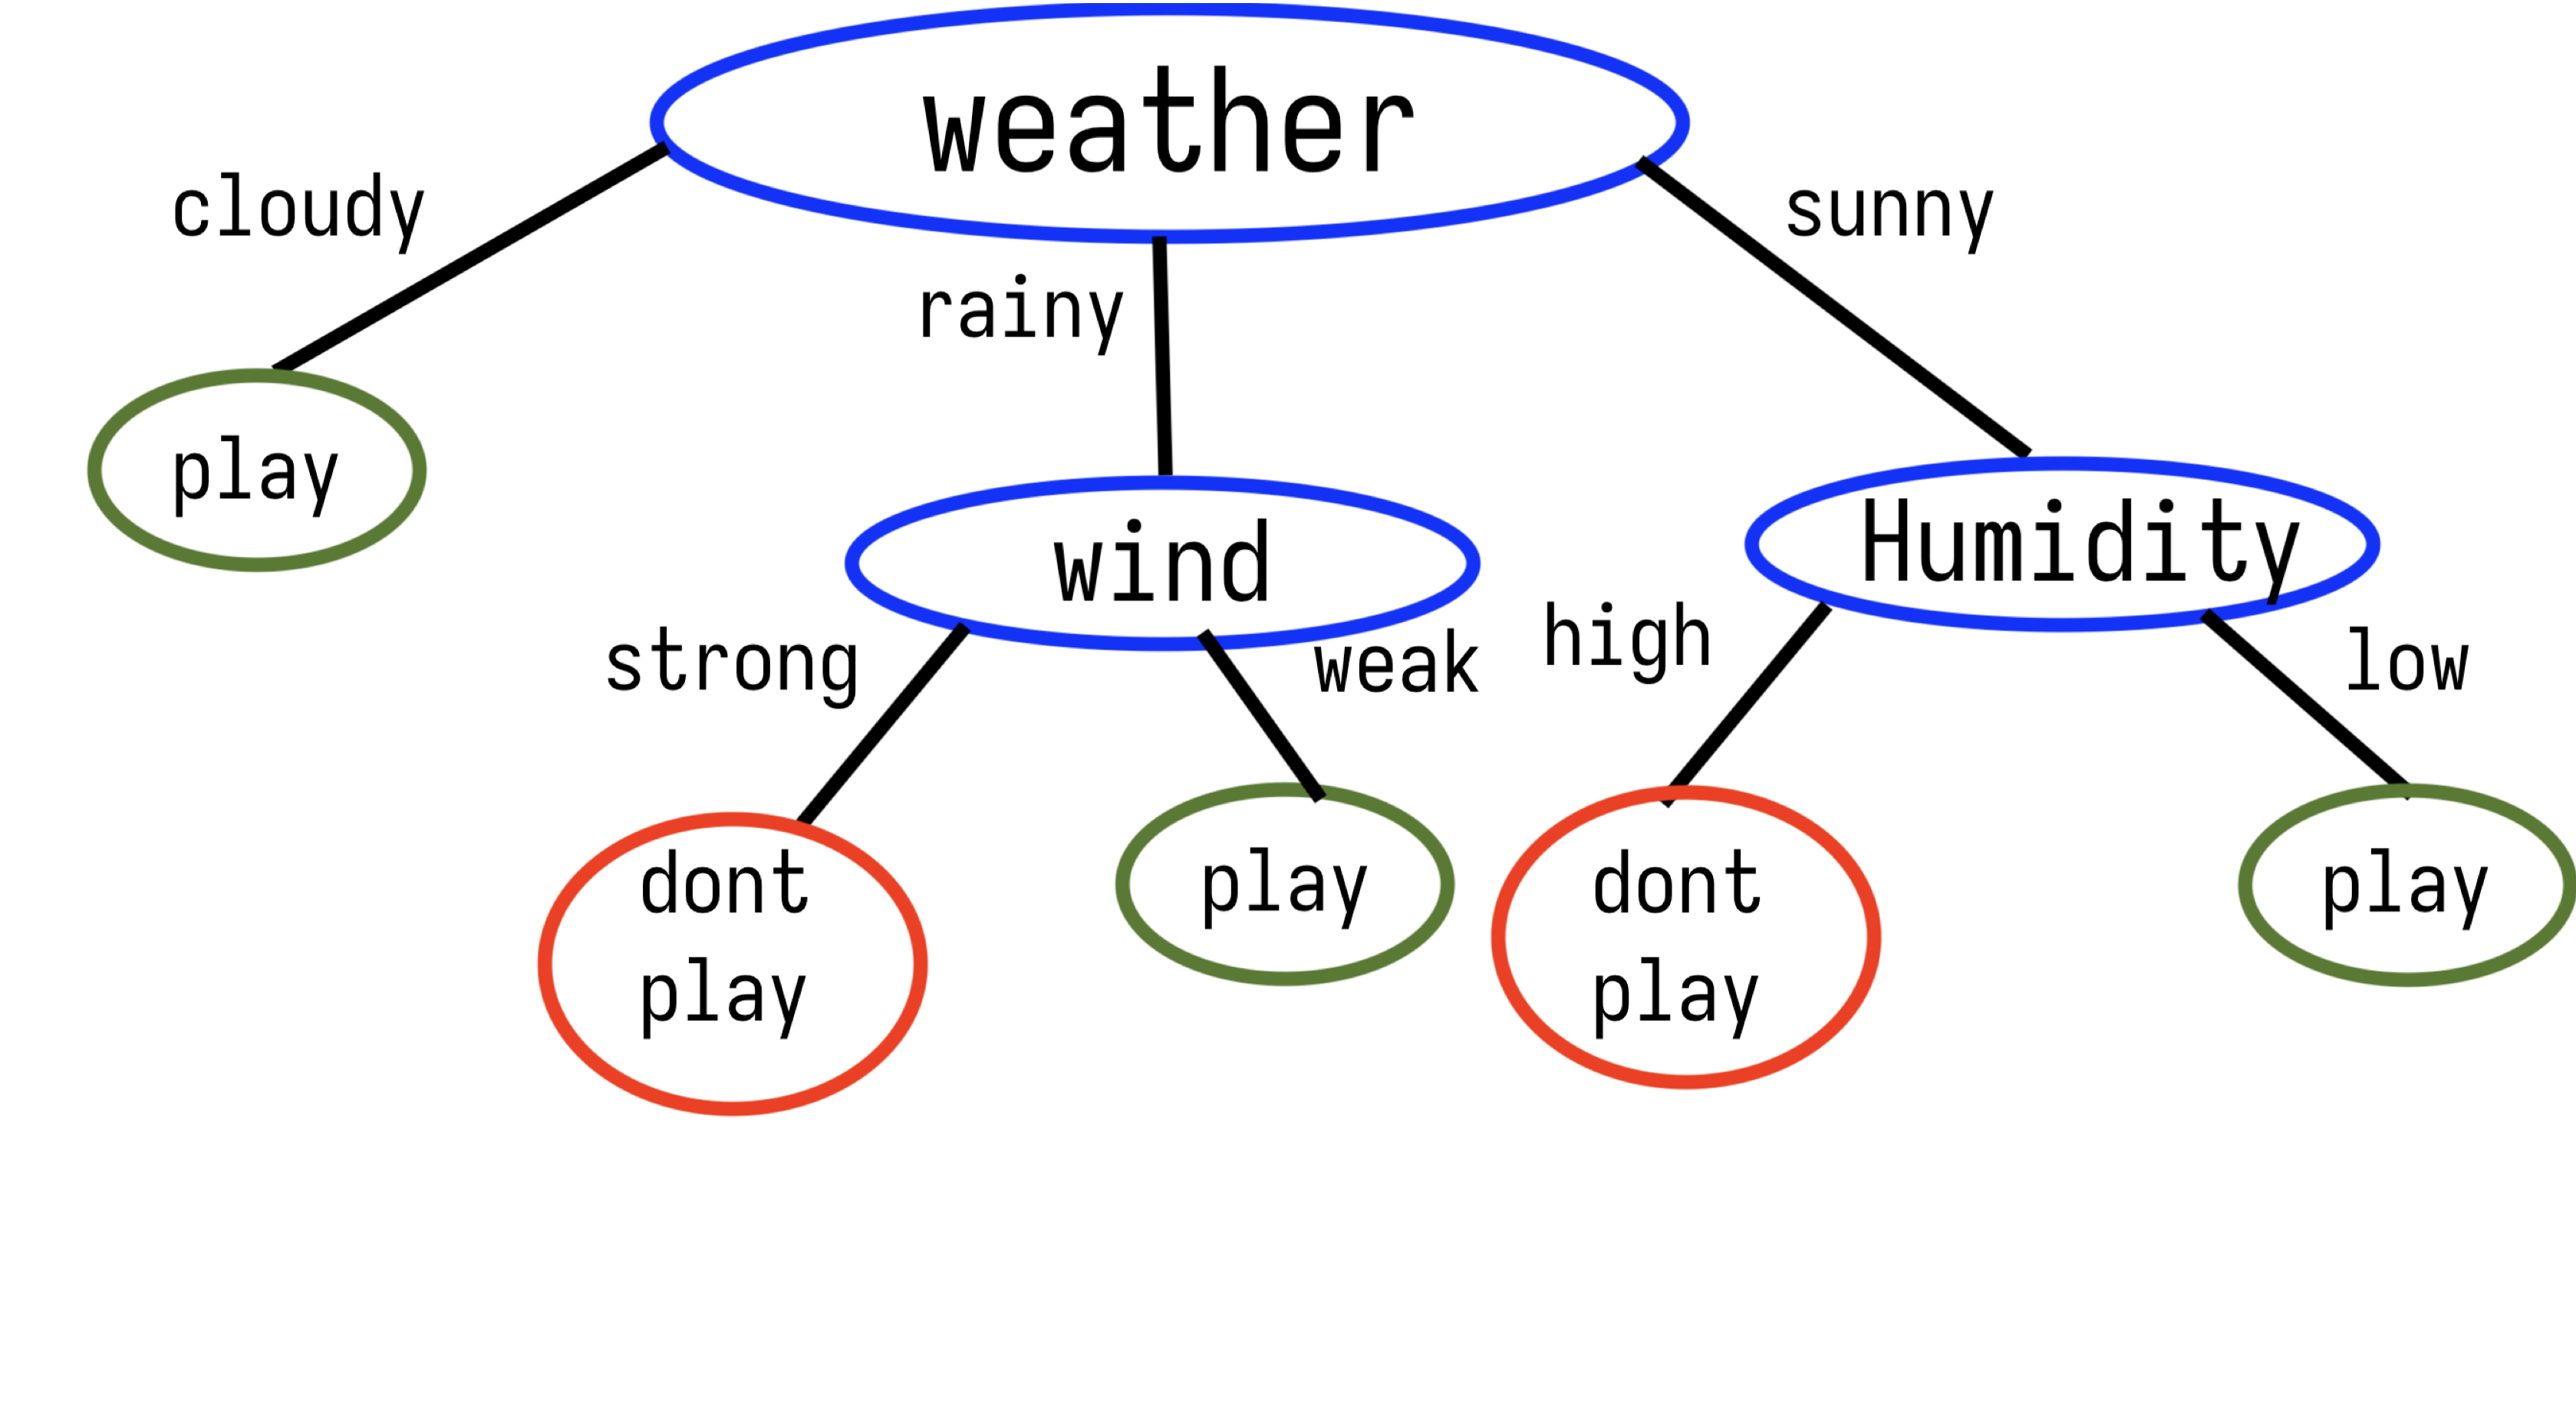
\includegraphics[width=0.8\textwidth]{2.png}
\end{center}

\subsection*{1.3 Pruning (Extra Points)}

mrleebc1

\section*{2. Perceptron}
\subsection*{2.1 Single Data Point}
With a step size of $1$, it will always take $\textbb{one}$ iteration to classify the data point.

\subsection*{2.2 Random Initialization}
Given a randomly initialized weight vector, if $w_0$ correctly classifies the point, then $0$ iterations will be required, otherwise, we must consider another case: 

\subsection*{2.3 Iterative Updates}

\section*{3. Gaussian Discriminant Analysis (GDA)}

\subsection*{3.1 Estimating Parameters}
\begin{table}[h!]
\centering
\begin{tabular}{|c|c|c|}
\hline
\textbf{Class} & \textbf{Mean (\(\mu\))} & \textbf{Variance (\(\sigma^2\))} \\ \hline
Class +1       & -0.0722                 & 1.3031                          \\ \hline
Class -1       & 0.9402                  & 1.9426                          \\ \hline
\end{tabular}
\caption{Mean and variance for each class.}
\label{tab:class_stats}
\end{table}

\subsection*{3.2 Test Accuracy}
The test accuracy is 61\%

\subsection*{3.3 Improving the Classifier}
As currently constructed, we use MLE estimation. MLE only looks at likelihood and ignores prior probabilities. Using MAP rule, we can increase our effectiveness. With MAP, accuracy went up to 90\%

\subsection*{3.4 2D GDA Statistics}

\begin{table}[h!]
\centering
\begin{tabular}{|c|c|c|}
\hline
\textbf{Class} & \textbf{Mean (\(\mu\))} & \textbf{Covariance (\(\Sigma\))} \\ \hline
Class +1       & \([0.0130754, 0.06295251]\) & 
\(\begin{bmatrix}
0.98285498 & 0.00612046 \\ 
0.00612046 & 1.05782804 
\end{bmatrix}\) \\ \hline
Class -1       & \([-0.02313942, -0.02114952]\) & 
\(\begin{bmatrix}
1.00329037 & -0.01142356 \\ 
-0.01142356 & 4.97693356 
\end{bmatrix}\) \\ \hline
\end{tabular}
\caption{Mean and covariance for each class.}
\label{tab:class_stats}
\end{table}

\subsection*{3.5 2D GDA Predictions}
The test accuracy is 84\%

\subsection*{3.6 Density-Based Accuracy (Extra Points)}
The test accuracy is 85\% which shows us that GDA is suitable. GDA provides a reasonable framework for classification because it balances robustness, simplicity, and efficiency, achieving near-optimal accuracy even when the data deviates slightly from Gaussian assumptions. A more complex mixture model wasn't that much of an improvement.

\section*{4. Logistic Regression}
\subsection*{4.1 Data Preprocessing}
\subsection*{4.2 Dimensionality Reduction}
\subsection*{4.3 Gradient Descent}
\subsection*{4.4 Train and Test Accuracy}
\subsection*{4.5 Extra Points: Email Classification}

\end{document}
